\documentclass[letterpaper,12pt]{article}
\usepackage{bookmark}
\usepackage[utf8]{inputenc}
\usepackage[spanish,es-tabla]{babel}
\usepackage{amsfonts}
\usepackage{graphicx}
\usepackage{mathptmx}
\usepackage{float}
\usepackage[T1]{fontenc}
\usepackage[margin=1.3in]{geometry}
\usepackage{amsthm}
\usepackage{marvosym}
\usepackage{bm}



\renewcommand\qedsymbol{\Squarepipe}

\theoremstyle{definition}
\newtheorem{definition}{Definición}[section]
\newtheorem*{thm}{Teorema}


\setlength\parindent{0pt}

\newcounter{paragraphnumber}
\newcommand{\para}{%
  \vspace{10pt}\noindent{\bfseries\refstepcounter{paragraphnumber}\theparagraphnumber.\quad}%
}

%\setsecheadstyle{\large\bfseries}
%\setsubsecheadstyle{\bfseries}

\setlength\parindent{0pt}

\pagenumbering{gobble}

%\usepackage[margin=1in]{geometry}

\usepackage{enumitem}
\setlist{nosep}

\usepackage{xcolor}
\usepackage{booktabs} 
\usepackage{colortbl} 
\usepackage{xfrac}

%\newcommand{ra}[1]{renewcommand{arraystretch}{#1}}


\usepackage{hyperref}
\hypersetup{
  colorlinks,
  linkcolor={red!50!black},
  citecolor={blue!50!black},
  urlcolor={green!50!black}
}

\usepackage{amssymb}
\usepackage{amsmath}

\begin{document}

\begin{center}
  {\large Cómputo Evolutivo}\\
  \vspace{0.2cm}
  {\large\bfseries Tarea 2}\\
  \vspace{0.2cm}
  {\large PCIC - UNAM}\\
  \vspace{0.5cm}
  {\itshape 4 de marzo de 2020}\\
  \vspace{0.5cm}
  Diego de Jesús Isla López\\
  (\href{mailto:dislalopez@gmail.com}{\itshape dislalopez@gmail.com})\\
  (\href{mailto:diego.isla@comunidad.unam.mx}{\itshape diego.isla@comunidad.unam.mx})\\
\end{center}



\section{Definición del problema}

Utilizar el algoritmo genético con codificaciones binaria, real y entera para resolver los problemas de N-reinas y agente viajero (TSP). Se mantienen los siguientes parámetros\\

\begin{itemize}
  \item Selección: Torneo binario
  \item Cruza: aleatoria en un punto con tasa de \(0.9\)
  \item Mutación: aleatoria con tasa de \(\frac{0.1}{L}\) donde \(L\) es la longitud del individuo
  \item Elitismo
  \item Población: \(100\) individuos
  \item Número de generaciones: \(500\)
\end{itemize}

\medskip

La instancia de TSP a resolver es GR17\footnote{Disponible en \url{https://people.sc.fsu.edu/~jburkardt/datasets/tsp/tsp.html}}, por lo que la dimensión es de 17 variables. Por su parte, las pruebas para N-reinas se harán con \(n = 8\).


\section{Función de aptitud}

En el caso de N-reinas, el problema se centra en reducir el número de ataques. Para el caso de TSP, se busca el ciclo más corto para el recorrido de todas las ciudades regresando al punto de inicio. Como se describe en la documentación del problema, para la instancia GR17 la distancia óptima es 2085.

\section{Resultados}

Las gráficas muestran el desempeño de 10 ejecuciones para cada instancia, siendo la evolución de la mejor solución a lo largo de las generaciones.

\subsection{Codificación entera}

En el caso de N-reinas, el desempeño de algoritmo es contundente pues logra encontrar una solución factible en las primeras generaciones, la cual guía el resto de los resultados hasta el fin de la ejecución (figura \ref{fig:nqint}). Como es posible ver en la tabla \ref{tab:nqint}, el promedio de todas las ejecuciones es \(0.012\), lo que nos habla de un desempeño uniforme y encontrando soluciones factibles desde etapas tempranas de la ejecución del algoritmo. \\

\begin{figure}[H]
  
    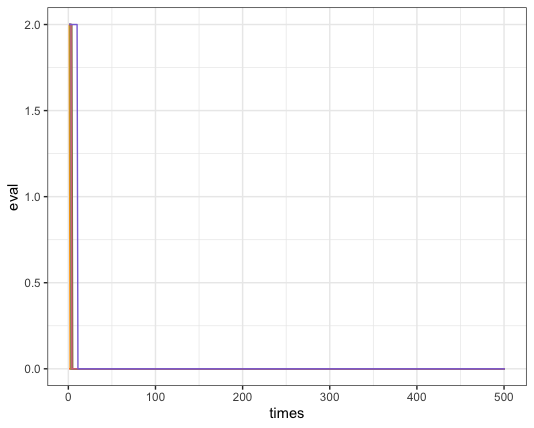
\includegraphics[width=\linewidth]{int_nq}
    \caption{Resultados para N-reinas con codificación entera}
    \label{fig:nqint}
\end{figure}

\begin{table}
  \begin{center}
    \begin{tabular}{cccc}
      \toprule 
        Muestra & \(\Sigma f(x)\) & \(\sigma\)  & \(\sigma^2\)  \\
        \midrule
        \rowcolor{black!20} E1 & 0 & 0 & 0 \\
        E2 & 4 & 0.1262384 & 0.01593613 \\
        \rowcolor{black!20} E3 & 2 & 0.08935341 & 0.007984032\\
        E4 & 6 & 0.1544548 & 0.02385629\\
        \rowcolor{black!20} E5 & 6 & 0.1544548 & 0.02385629 \\
        E6 & 6 & 0.1544548 & 0.02385629 \\
        \rowcolor{black!20} E7 & 4 & 0.1262384 & 0.01593613 \\
        E8 & 8 & 0.1781699 & 0.03174451\\
        \rowcolor{black!20} E9 & 6 & 0.1544548 & 0.02385629 \\
        E10 & 20 & 0.2800057 & 0.07840319 \\
        \rowcolor{black!20} \(\mu\) & 0.012 & 0.1566618 & 0.02454291 \\ 
        \bottomrule
      \end{tabular}
  \end{center}
  \caption{Análisis estadístico de las ejecuciones de N-reinas en codificación entera}
  \label{tab:nqint}  
\end{table}

En el caso del problema TSP, se puede observar que en promedio el desempeño es bueno y con tendencia a acercarse a la solución óptima (figura \ref{fig:tspint}). En la tabla \ref{tab:tspint} podemos constatar que el promedio de las soluciones es muy cercano al óptimo, con una desviación estándar relativamente pequeña, lo que concuerda con lo visto en la gráfica. 

\begin{table}
  \begin{center}
    \begin{tabular}{cccc}
      \toprule 
        Muestra & \(\Sigma f(x)\) & \(\sigma\)  & \(\sigma^2\)  \\
        \midrule
        \rowcolor{black!20} E1 & 1066757 & 149.9581 & 22487.44 \\
        E2 & 1061105 & 137.9094 & 19019 \\
        \rowcolor{black!20} E3 & 1089541 & 148.3441 & 22005.97\\
        E4 & 1067960 & 119.5627 & 14295.24\\
        \rowcolor{black!20} E5 & 1065858 & 126.6666 & 16044.42 \\
        E6 & 1065931 & 120.611 & 14547.02 \\
        \rowcolor{black!20} E7 & 1092353 & 139.7941 & 19542.38 \\
        E8 & 1073028 & 155.7204 & 24248.85\\
        \rowcolor{black!20} E9 & 1063132 & 158.0054 & 24965.7 \\
        E10 & 1090362 & 146.0115 & 21319.37 \\
        \rowcolor{black!20} \(\mu\) & 2138.65 & 140.8813 & 19847.54 \\ 
        \bottomrule
      \end{tabular}
  \end{center}
  \caption{Análisis estadístico de las ejecuciones de TSP en codificación entera}
  \label{tab:tspint}  
\end{table}


\begin{figure}[H]
  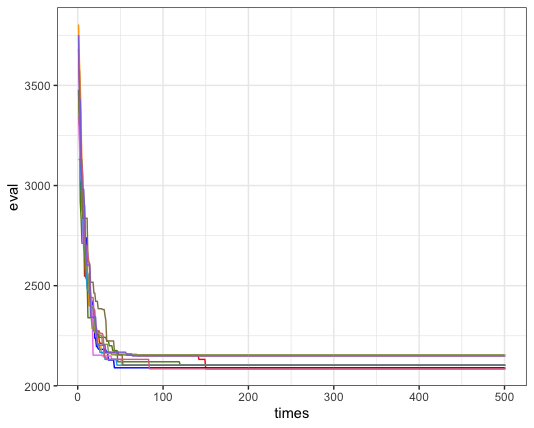
\includegraphics[width=\linewidth]{int_tsp}
  \caption{Resultados para TSP con codifcación entera}
  \label{fig:tspint}
\end{figure}


\subsection{Codificación real}

En el caso de N-reinas, podemos observar en la figura \ref{fig:nqreal} que el comportamiento tiene una tendencia clara a minimizar, sin embargo la mayoría de las ejecuciones no pudieron mejorar más allá de 2 colisiones, siendo solo una ejecución en la que se llegó al óptimo de 0 colisiones. En la tabla \ref{tab:nqreal} podemos constatar esto, viendo que el promedio es 1.94 con una desviación estándar mínima.

\begin{table}
  \begin{center}
    \begin{tabular}{cccc}
      \toprule 
        Muestra & \(\Sigma f(x)\) & \(\sigma\)  & \(\sigma^2\)  \\
        \midrule
        \rowcolor{black!20} E1 & 1018 & 0.2509543 & 0.0629780 \\
        E2 & 1026 & 0.4355463 & 0.1897006 \\
        \rowcolor{black!20} E3 & 1098 & 0.7233323 & 0.5232096\\
        E4 & 1062 & 0.6585049 & 0.4336287\\
        \rowcolor{black!20} E5 & 1114 & 0.9197414 & 0.8459242 \\
        E6 & 1028 & 0.4441862 & 0.19730149 \\
        \rowcolor{black!20} E7 & 1102 & 0.8989326 & 0.8080798 \\
        E8 & 1062 & 0.6939948 & 0.4816287\\
        \rowcolor{black!20} E9 & 80 & 0.9156698 & 0.8384511 \\
        E10 & 1170 & 1.193034 & 1.423329 \\
        \rowcolor{black!20} \(\mu\) & 1.94 & 0.7618551 & 0.5804232 \\ 
        \bottomrule
      \end{tabular}
  \end{center}
  \caption{Análisis estadístico de las ejecuciones de N-reinas en codificación real}
  \label{tab:nqreal}  
\end{table}

\begin{figure}[H]
  
  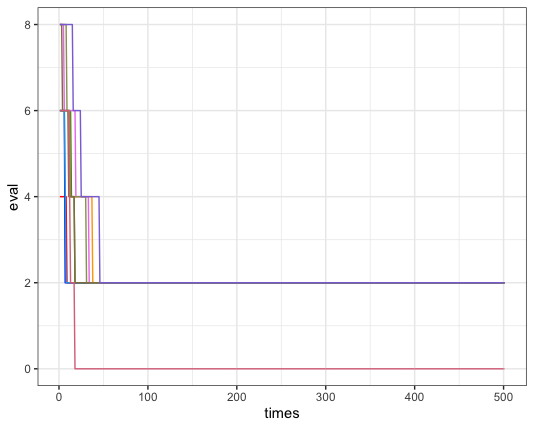
\includegraphics[width=\linewidth]{real_nq}
  \caption{Resultados para N-reinas con codificación real}
  \label{fig:nqreal}
\end{figure}

El caso de TSP es interesante, ya que la codificación real no dio buenos resultados. A pesar de que en la gráfica podemos observar un comportamiento estable (figura \ref{fig:tspreal}), las soluciones generadas presentan valores repetidos y esto se refleja en el valor de la función objetivo, el cual se minimiza más allá del valor óptimo conocido (tabla \ref{tab:tspreal}).

\begin{table}
  \begin{center}
    \begin{tabular}{cccc}
      \toprule 
        Muestra & \(\Sigma f(x)\) & \(\sigma\)  & \(\sigma^2\)  \\
        \midrule
        \rowcolor{black!20} E1 & 275240 & 290.7977 & 84563.31 \\
        E2 & 279838 & 278.9088 & 77790.09 \\
        \rowcolor{black!20} E3 & 152446 & 275.7725 & 76050.46\\
        E4 & 120820 & 264.9394 & 70192.89\\
        \rowcolor{black!20} E5 & 233835 & 296.5924 & 87967.05 \\
        E6 & 158908 & 311.4078 & 96974.79 \\
        \rowcolor{black!20} E7 & 277379 & 218.9546 & 47941.11 \\
        E8 & 171000 & 270.4682 & 73153.03\\
        \rowcolor{black!20} E9 & 335679 & 227.414 & 51717.15 \\
        E10 & 152217 & 285.1013 & 81282.74 \\
        \rowcolor{black!20} \(\mu\) & 429.75 & 258.8132 & 74763.26 \\ 
        \bottomrule
      \end{tabular}
  \end{center}
  \caption{Análisis estadístico de las ejecuciones de TSP en codificación real}
  \label{tab:tspreal}  
\end{table}

\begin{figure}[H]
  
  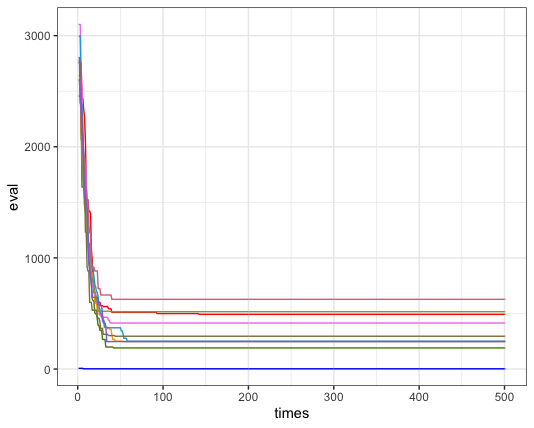
\includegraphics[width=\linewidth]{real_tsp}
  \caption{Resultados para TSP con codificación real}
  \label{fig:tspreal}
\end{figure}


\subsection{Codificación binaria}

Para estas ejecuciones se usó el método de codificación propuesto en \cite{moh06} en la que se mapea cada combinación válida a una cadena binaria. \\

En el caso de N-reinas observamos un desempeño en el que rápidamente se encuentran soluciones factibles y se mantienen durante el resto de la ejecución (figura \ref{fig:nqbinaria}), incluso habiendo una ejecución donde desde el inicio se encontraron solo soluciones factibles. Podemos corroborar en la tabla \ref{tab:nqbin} que el promedio de las soluciones es 0 con una desviación estándar casi nula.

\begin{table}
  \begin{center}
    \begin{tabular}{cccc}
      \toprule 
        Muestra & \(\Sigma f(x)\) & \(\sigma\)  & \(\sigma^2\)  \\
        \midrule
        \rowcolor{black!20} E1 & 8 & 0.1781698936 & 0.03174451098 \\
        E2 & 2 & 0.08935341032 & 0.007984031936 \\
        \rowcolor{black!20} E3 & 0 & 0 & 0\\
        E4 & 0 & 0 & 0\\
        \rowcolor{black!20} E5 & 2 & 0.08935341032 & 0.007984031936 \\
        E6 & 0 & 0 & 0 \\
        \rowcolor{black!20} E7 & 0 & 0 & 0 \\
        E8 & 4 & 0.1262383767 & 0.01593612774\\
        \rowcolor{black!20} E9 & 0 & 0 & 0 \\
        E10 & 0 & 0 & 0 \\
        \rowcolor{black!20} \(\mu\) & 0.003 & 0.07978014 & 0.00636487 \\ 
        \bottomrule
      \end{tabular}
  \end{center}
  \caption{Análisis estadístico de las ejecuciones de N-reinas en codificación binaria}
  \label{tab:nqbin}  
\end{table}

\begin{figure}[H]
  
  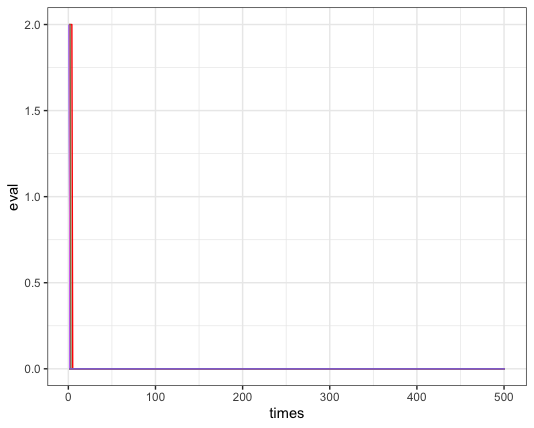
\includegraphics[width=\linewidth]{bin_nq}
  \caption{Resultados para N-reinas con codificación binaria}
  \label{fig:nqbinaria}
\end{figure}

En el caso de TSP, tenemos un desempeño regular, con tendencia a optimizar el valor de las soluciones (figura \ref{fig:tspbinaria}), sin embargo solo en dos ejecuciones se llega al valor óptimo. En la tabla \ref{tab:tspbin} podemos observar que el promedio está en 2663.95 con una desviación estándar de 59.74, lo que nos hace corroborar el comportamiento estable ya mencionado.

\begin{table}
  \begin{center}
    \begin{tabular}{cccc}
      \toprule 
        Muestra & \(\Sigma f(x)\) & \(\sigma\)  & \(\sigma^2\)  \\
        \midrule
        \rowcolor{black!20} E1 & 1478086 & 29.73762 & 884.3262 \\
        E2 & 1307335 & 56.70072 & 3214.972 \\
        \rowcolor{black!20} E3 & 1351190 & 33.31777 & 1110.074\\
        E4 & 1331309 & 33.90026 & 1149.228\\
        \rowcolor{black!20} E5 & 1263318 & 48.51773 & 2353.97 \\
        E6 & 1236899 & 107.0594 & 11461.72 \\
        \rowcolor{black!20} E7 & 1512827 & 6.85954 & 47.0533 \\
        E8 & 1220855 & 78.90086 & 6225.345\\
        \rowcolor{black!20} E9 & 1329707 & 77.87225 & 6064.087 \\
        E10 & 1341517 & 56.4382 & 3185.271 \\
        \rowcolor{black!20} \(\mu\) & 2663.95 & 59.74617 & 3569.605 \\ 
        \bottomrule
      \end{tabular}
  \end{center}
  \caption{Análisis estadístico de las ejecuciones de TSP en codificación binaria}
  \label{tab:tspbin}  
\end{table}

\begin{figure}[H]
  
  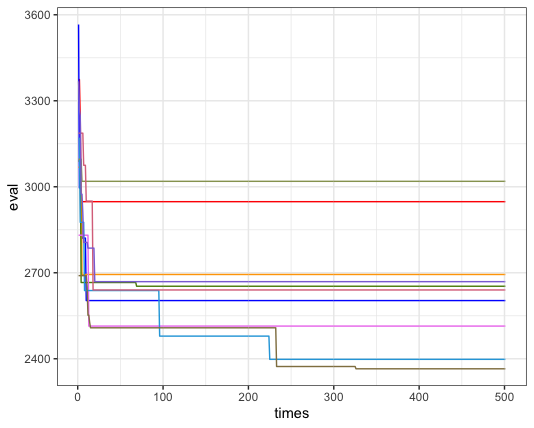
\includegraphics[width=\linewidth]{bin_tsp}
  \caption{Resultados para TSP con codificación binaria}
  \label{fig:tspbinaria}
\end{figure}

\section{Conclusiones}

Los mejores resultados para ambos casos de los problemas se obtuvieron utilizando la codificación entera, donde se encontraron valores óptimos en los dos problemas. Es posible apreciar cómo al utilizar la codificación binaria, es posible encontrar buenos resultados para ambos problemas; sin embargo, en el caso de TSP es notoria la dificultad que tiene el algoritmo para encontrar la solución óptima. Es de hacer notar el desempeño presentado con TSP en la codificación real; este comportamiento puede estar relacionado con la precisión usada para representar cada valor del conjunto.

\bibliography{references}
\bibliographystyle{unsrt}



\end{document}